\documentclass[tikz,border=8pt]{standalone}
\usepackage{amsmath}
\usetikzlibrary{arrows.meta,calc}
\definecolor{ink}{HTML}{21352F}
\definecolor{teal}{HTML}{087F7B}
\definecolor{blue}{HTML}{4B77A8}
\definecolor{gold}{HTML}{C58B2A}
\definecolor{rose}{HTML}{B65A62}
\begin{document}
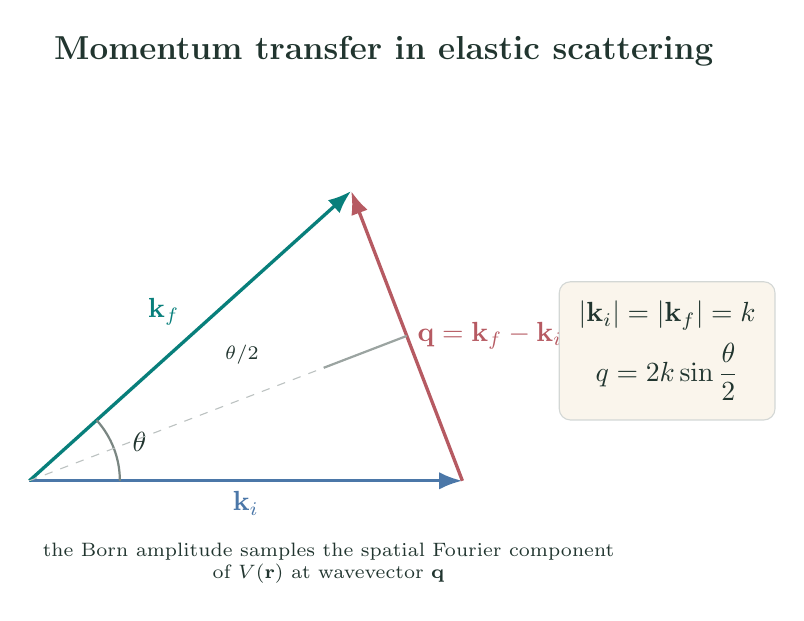
\begin{tikzpicture}[font=\sffamily,text=ink,>=Latex]
  \node[font=\bfseries\large] at (0,3.9)
    {Momentum transfer in elastic scattering};
  \coordinate (O) at (-4.5,-1.55);
  \coordinate (I) at (1.0,-1.55);
  \coordinate (F) at ($(O)+(42:5.5)$);

  \draw[blue,very thick,->] (O)--(I)
    node[midway,below] {$\mathbf k_i$};
  \draw[teal,very thick,->] (O)--(F)
    node[midway,above left] {$\mathbf k_f$};
  \draw[rose,very thick,->] (I)--(F)
    node[midway,right] {$\mathbf q=\mathbf k_f-\mathbf k_i$};

  \draw[ink!60,thick] ($(O)+(1.15,0)$)
    arc[start angle=0,end angle=42,radius=1.15];
  \node at (-3.1,-1.05) {$\theta$};
  \draw[ink!30,dashed] (O)--($(O)+(21:5.1)$);
  \node[font=\scriptsize] at (-1.8,.05) {$\theta/2$};

  \draw[ink!45,thick]
    ($(I)!0.5!(F)$)--($(O)!0.78!($(I)!0.5!(F)$)$);
  \node[draw=ink!20,fill=gold!9,rounded corners=4pt,
        inner sep=7pt,align=center] at (3.6,.1)
    {$|\mathbf k_i|=|\mathbf k_f|=k$\\[4pt]
     $\displaystyle q=2k\sin\frac{\theta}{2}$};

  \node[font=\scriptsize,align=center] at (-.7,-2.6)
    {the Born amplitude samples the spatial Fourier component\\
     of $V(\mathbf r)$ at wavevector $\mathbf q$};
\end{tikzpicture}
\end{document}
